% 附录 V：破裂、误差场与逃逸电子（v1.19.0 新增）
% 数值唯一来源：tools/calc/appV_calc.py -> tools/calc/appV_calc.txt（正文数字的唯一来源；检查项 P26）
% 时间单位写成 s/ms，避免中文字符进入数学字体；全部数字可用仓库脚本复算。
% 版权口径：只借鉴经典教材与文献的物理结论、公式形式与题型；文字、数值与表格自拟并独立复算。
% 本书不列 DOI，只给书名、作者、年份、卷期页。
% 分工：M 管加热与运行极限的"面"，N 管边界与瞬态热负荷，S 管约束，T 管拓扑里的磁岛，
% U 管增益与点火；本附录管"运行空间什么时候被撞破"，并把它们串成一条时间线。

\section{破裂：三张极限图与一条时间线}
\label{sec:app-v-what}

第 10 章讲点火，附录 M 讲加热与运行极限，附录 S 把约束写成一个数 $\tau_E$，附录 U 把增益
算到电功率。这些讨论都默认一件事：放电能一直持续下去。破裂（disruption）就是把这个默认
拿掉：等离子体在毫秒尺度上失去约束，把热储能与电流在很短时间内交给第一壁。

先看工作点站在三张极限图里的位置。沿用附录 S 与附录 U 的 D1（ITER 量级）点：
$n=10^{20}\ \mathrm{m^{-3}}$、$T=9.194\ \mathrm{keV}$、$B=5.3\ \mathrm{T}$、
$a=2.0\ \mathrm{m}$、$I_{\mathrm p}=15\ \mathrm{MA}$。

\begin{equation}
\beta = \frac{2\mu_0 n k_B T}{B^2} = 2.6359\%,
\qquad
\beta_N \equiv \frac{\beta\,[\%]\;a\,[\mathrm{m}]\;B\,[\mathrm{T}]}{I_{\mathrm p}\,[\mathrm{MA}]}
= 1.8627
\label{eq:app-v-betan}
\end{equation}

\begin{equation}
n_G = \frac{I_{\mathrm p}\,[\mathrm{MA}]}{\pi a^2}\times10^{20}\ \mathrm{m^{-3}}
= 1.1937\times10^{20}\ \mathrm{m^{-3}},
\qquad
\frac{n}{n_G} = 83.78\%
\label{eq:app-v-greenwald}
\end{equation}

两条式子都说明 D1 点并不宽松：$\beta_N$ 已经用掉无壁极限的相当一部分（V.3 再算裕度），
密度则用掉 Greenwald 极限的 $83.78\%$。这与附录 M、附录 U 用的是同一个 $n_G$ 口径。

破裂不是一种故障，而是五条不同路径通向同一个结局。表 \ref{tab:app-v-limits} 把它们并排
列出：注意每条路径都有自己的先兆信号，工程上正是靠这些信号争取那几十毫秒。

\begin{table}[htbp]
\centering
\small
\caption{破裂的五条常见路径。五条路径的先兆不同，但结局都是热猝灭加电流猝灭；本附录
把结局的账算在表 \ref{tab:app-v-timeline}。}
\label{tab:app-v-limits}
\begin{tabular}{@{}p{2.6cm}p{3.9cm}p{3.2cm}p{3.4cm}@{}}
\toprule
撞破的极限 & 物理机制 & 先兆信号 & 本书哪一节讲过 \\
\midrule
密度极限 & 边缘辐射与脱靶使辐射崩塌，电流剖面收缩 & 辐射功率骤升、约束变差 & 附录 M、附录 U（$n_G=1.1937\times10^{20}$） \\
$\beta$ 极限 & 理想 MHD 外扭曲模失稳（无壁 2.8 / 理想壁 4.0） & 低频 $n=1$ 磁扰动 & 附录 S（$\beta_N$）、本附录 V.3 \\
误差场锁模 & 静态 $m/n$ 场误差在有理面上生成磁岛并锁定 & 锁模信号、旋转下降 & 附录 T（磁岛）、本附录 V.2 \\
杂质积累 & 高 $Z$ 杂质聚芯，辐射超过加热 & 辐射剖面峰化、$Z_{\mathrm{eff}}$ 上升 & 附录 N（杂质与脱靶） \\
垂直位移 & 拉长截面的垂直不稳定，等离子体撞向壁 & 垂直位置漂移、$I_{\mathrm p}$ 变化 & 本附录 V.4（晕电流） \\
\bottomrule
\end{tabular}

\end{table}

\begin{table}[htbp]
\centering
\small
\caption{一次破裂的时间线。五个阶段不是五个独立事件，而是同一笔能量账在五个时间尺度上的
展开；表里的数字分别由 V.5、V.4、V.6 的公式复算。}
\label{tab:app-v-timeline}
\begin{tabular}{@{}p{2.4cm}p{2.5cm}p{3.8cm}p{4.3cm}@{}}
\toprule
阶段 & 时长 & 这一段时间里发生了什么 & 数字 \\
\midrule
先兆 & $10$--$100\ \mathrm{ms}$ & 锁模或辐射异常出现，控制系统开始判断 & 经验统计窗口（V.6 声明） \\
热猝灭 & $\sim1\ \mathrm{ms}$ & 磁面被破坏，热储能沿开磁力线泄到壁 & $371.4\ \mathrm{MJ}$ 在 $1\ \mathrm{ms}$ 内是 $371.4\ \mathrm{GW}$ \\
电流猝灭 & $50$--$150\ \mathrm{ms}$ & 电流靠等离子体电阻衰减，环电压飙升 & $T_e=10\ \mathrm{eV}$ 给 $\tau_{\mathrm{CQ}}=76.9074\ \mathrm{ms}$、$V_{\mathrm{loop}}=2600\ \mathrm{V}$ \\
晕电流 & 与电流猝灭同时 & 开磁力线把电流引到壁，形成不对称的晕电流 & $I_{\mathrm{halo}}=4.5\ \mathrm{MA}$，力约 $79.5\ \mathrm{MN}$ \\
逃逸平台 & $100\ \mathrm{ms}$--$1\ \mathrm{s}$ & 高能电子尾巴雪崩，束带着几 MA 电流继续跑 & $26.0\ \mathrm{MJ}$，落在 $0.1\ \mathrm{m^2}$ 上是 $259.9\ \mathrm{MJ/m^2}$ \\
\bottomrule
\end{tabular}

\end{table}

\begin{tip}{破裂是一条时间线，不是一个事件}{tip-app-v-timeline}
记住本附录要算的四个时间尺度：壁的 $\tau_w=52.7788\ \mathrm{ms}$（V.3）、雪崩的
$\tau_{\mathrm{av}}=0.4342\ \mathrm{ms}$（V.5）、电流猝灭的 $76.9074\ \mathrm{ms}$
（V.4）、反馈必须达到的 $189.47\ \mathrm{s^{-1}}$（V.3）。破裂物理的核心问题因此是「谁更快」：
如果雪崩比电流猝灭快两个量级，那么「把电流快速拉掉」这条路本身就会先催出逃逸电子。
\end{tip}

{\footnotesize
\textbf{出处：} 三条运行极限（密度、$\beta$、误差场）的分类与破裂的时间线参照 Wesson
《Tokamaks》第 4 版（Oxford, 2011）第 14 章与 Freidberg《Plasma Physics and Fusion
Energy》（Cambridge, 2007）第 13 章，以及 Hender 等（2007）\textit{Nucl.\ Fusion}
\textbf{47}, S128（ITER Physics Basis 第 3 章）。工作点上的 $\beta$、$\beta_N$、$n_G$
由
}

\section{误差场与锁模：万分之一的场误差如何吃掉运行空间}
\label{sec:app-v-errorfield}

附录 T 讲过一件事：有理面上的磁岛由垂直场误差驱动。真实装置里，这个误差有一部分是「自找
的」。线圈引线、母线、铁磁部件与线圈安装偏差都会产生一个静态的非轴对称场。它不需要很大，
就足以把运行空间切掉一块。

先把「场误差在真空里怎么随半径变化」算清楚。对单个极向模数 $m$ 的静态扰动，真空中的通量
函数满足 $\nabla^2\psi-(m^2/r^2)\psi=0$，在壁以内满足正则性的解是 $\psi\propto r^m$，
于是垂直场按 $r^{m-1}$ 变化：

\begin{equation}
\frac{B_r(r_s)}{B_r(r_w)} = \left(\frac{r_s}{r_w}\right)^{m-1}
\label{eq:app-v-vacuum}
\end{equation}

取壁半径 $r_w=1.2a=2.4\ \mathrm{m}$、$q=2$ 面在 $r_s=0.8a=1.6\ \mathrm{m}$：$m=2$ 分量
从壁到该面衰减到 $0.6667$；$m=3$ 分量在 $r_s=0.9a=1.8\ \mathrm{m}$ 上衰减到 $0.5625$。
这是\textbf{真空}衰减，不是等离子体响应：真实的等离子体会把共振分量再放大，所以壁上的
允许值比真空折算更小。

经验上，$m/n=2/1$ 分量在 $q=2$ 面上达到 $\delta B/B\approx10^{-4}$ 就会锁模。把它按式
\eqref{eq:app-v-vacuum} 折回壁面：允许的静态误差升到 $1.5\times10^{-4}$，用
$B_t=5.3\ \mathrm{T}$ 换算就是 $0.795\ \mathrm{mT}$。表 \ref{tab:app-v-errorfield} 把两个
分量的折算并列出来。

\begin{table}[htbp]
\centering
\small
\caption{误差场从壁面到有理面的真空折算（$r_w=2.4\ \mathrm{m}$）。阈值取
$\delta B/B\approx10^{-4}$（$q=2$ 面上的经验锁模阈值），绝对场按 $B_t=5.3\ \mathrm{T}$
换算。}
\label{tab:app-v-errorfield}
\begin{tabular}{@{}p{2.3cm}p{2.1cm}p{2.5cm}p{3.0cm}p{3.1cm}@{}}
\toprule
分量 & $r_s$ [m] & $(r_s/r_w)^{m-1}$ & 折回壁面的 $\delta B/B$ & 绝对场（$B_t=5.3\ \mathrm{T}$） \\
\midrule
$m/n=2/1$ & 1.6 & 0.6667 & $1.5\times10^{-4}$ & $0.795\ \mathrm{mT}$ \\
$m/n=3/1$ & 1.8 & 0.5625 & $1.7778\times10^{-4}$ & $0.9422\ \mathrm{mT}$ \\
\bottomrule
\end{tabular}

\end{table}

锁模的下一半是力学。磁岛在旋转的等离子体里被粘性力矩带着转，误差场对它施加电磁力矩；
当旋转降到临界值以下，岛被「刹住」，就成了锁定模。

锁定的后果是连锁的：岛的宽度按附录 T 的岛宽公式增长，温度剖面被压平，储能下降。电流剖面
随之改变，密度极限下降，最终触发破裂。所以锁模是破裂最常见的先兆，现代装置都要装校正线圈：
ITER 的校正线圈是三组、每组六个（共 18 个），任务是把 $n=1$ 分量的静态误差压到阈值以下。

\begin{tip}{0.8 mT 有多小}{tip-app-v-errorfield}
$0.795\ \mathrm{mT}$ 大约是地磁场（$0.05\ \mathrm{mT}$）的 $15.9$ 倍，却只有一块普通钕铁硼
磁体表面场（约 $300\ \mathrm{mT}$）小两个多量级。所以误差场不是「加工精度问题」，而是一个
必须主动测量的运行参数：装置每次大修、部件更换之后都要重新测误差场，就是因为这个数太小。
\end{tip}

{\footnotesize
\textbf{出处：} 误差场的真空衰减规律与锁模的物理参照 Hender 等（2007）\textit{Nucl.\
Fusion} \textbf{47}, S128（ITER Physics Basis 第 3 章）与 Fitzpatrick（1993）
\textit{Nucl.\ Fusion} \textbf{33}, 1049（误差场穿透与锁定的理论）。
磁岛几何见本书附录 T。
本节的折算算例（$r_w=2.4\ \mathrm{m}$、两个分量）与全部数值为本书自拟。
}

\section{电阻壁模与 \texorpdfstring{$\beta$}{β} 极限：壁不是刚体}
\label{sec:app-v-rwm}

理想 MHD 给出一条很干净的分界：如果等离子体外围是一个理想导体壁，外扭曲模被完全稳定，
$\beta_N$ 可以做到 4.0；如果没有壁，只能做到 2.8。这两个数分别叫理想壁极限与无壁极限，
它们之间的空间不是「能不能」，而是「要多少控制」。

真实壁不是理想导体。磁场会以壁的 $L/R$ 时间常数扩散过去，这个时间叫壁时间：

\begin{equation}
\tau_w = \mu_0\,\sigma\,\delta\,d
\label{eq:app-v-tauw}
\end{equation}

其中 $\sigma$ 是壁的电导率、$\delta$ 是壁厚、$d$ 是壁到等离子体的特征距离。取
$\delta=3\ \mathrm{cm}$、$d=1\ \mathrm{m}$：不锈钢（$\sigma=1.4\times10^6\ \mathrm{S/m}$）
给 $\tau_w=52.7788\ \mathrm{ms}$，铜（$\sigma=5.8\times10^7\ \mathrm{S/m}$）给
$\tau_w=2.18655\ \mathrm{s}$。于是电阻壁模（RWM）只能被延迟，不能被抓死：

\begin{equation}
\gamma_{\mathrm{RWM}} \approx \frac{1}{\tau_w} = 18.947\ \mathrm{s^{-1}}
\label{eq:app-v-rwm}
\end{equation}

不锈钢壁给的是 $18.947\ \mathrm{s^{-1}}$ 的增长率。要让反馈系统在模长起来之前把它按住，
控制环路的带宽至少要到 $\tau_w/10$ 的时间尺度上，即 $189.47\ \mathrm{s^{-1}}$。这是「用线圈
和传感器把一个 MHD 模按住」的硬指标。

把两条极限折成温度，就能看出中间那块空间的价钱。固定 $n=10^{20}\ \mathrm{m^{-3}}$，
见表 \ref{tab:app-v-beta}。

\begin{table}[htbp]
\centering
\small
\caption{$\beta_N$ 极限折成的压力与温度（固定 $n=10^{20}\ \mathrm{m^{-3}}$）。理想壁极限
比无壁极限高 $1.4286$ 倍；工作点离无壁极限还有 $33.475\%$ 的裕度，但再往上走就必须靠
RWM 反馈把电阻壁「补」成理想壁。}
\label{tab:app-v-beta}
\begin{tabular}{@{}p{2.9cm}p{1.9cm}p{2.3cm}p{2.6cm}p{2.6cm}@{}}
\toprule
$\beta_N$ 极限 & $\beta$ [\%] & $p$ [Pa] & $T$（$n=10^{20}$）[keV] & 与工作点之比 \\
\midrule
无壁极限 2.8 & 3.9623 & $4.428\times10^{5}$ & 13.8202 & 1.503 \\
理想壁极限 4.0 & 5.6604 & $6.326\times10^{5}$ & 19.7432 & 2.147 \\
本书工作点 1.8627 & 2.6359 & $2.946\times10^{5}$ & 9.194 & 1.000 \\
\bottomrule
\end{tabular}

\end{table}

工作点的账是：$\beta_N=1.8627$，距无壁极限 2.8 还有 $33.475\%$ 的裕度，密度用掉 Greenwald
极限的 $83.78\%$。两条极限一条给「温度还能升多少」，一条给「密度还能加多少」，而它们并不独立：
提高密度会降低温度（功率平衡），提高温度则推高 $\beta$。运行空间就是这两条线之间的一块区域。

{\footnotesize
\textbf{出处：} $\beta_N$ 的定义与 Troyon 极限参照 Troyon 等（1984）\textit{Plasma
Phys.\ Control.\ Fusion} \textbf{26}, 209 与 Freidberg《Ideal MHD》（Cambridge, 2014）。
RWM 的物理与反馈控制参照 Chu \& Okabayashi（2010）\textit{Plasma Phys.\ Control.\
Fusion} \textbf{52}, 123001。
无壁与理想壁的数值区间见 Hender 等（2007）。$\tau_w$ 的
算例、增长率与反馈带宽要求为本书自拟。
}

\begin{figure}[htbp]
\centering
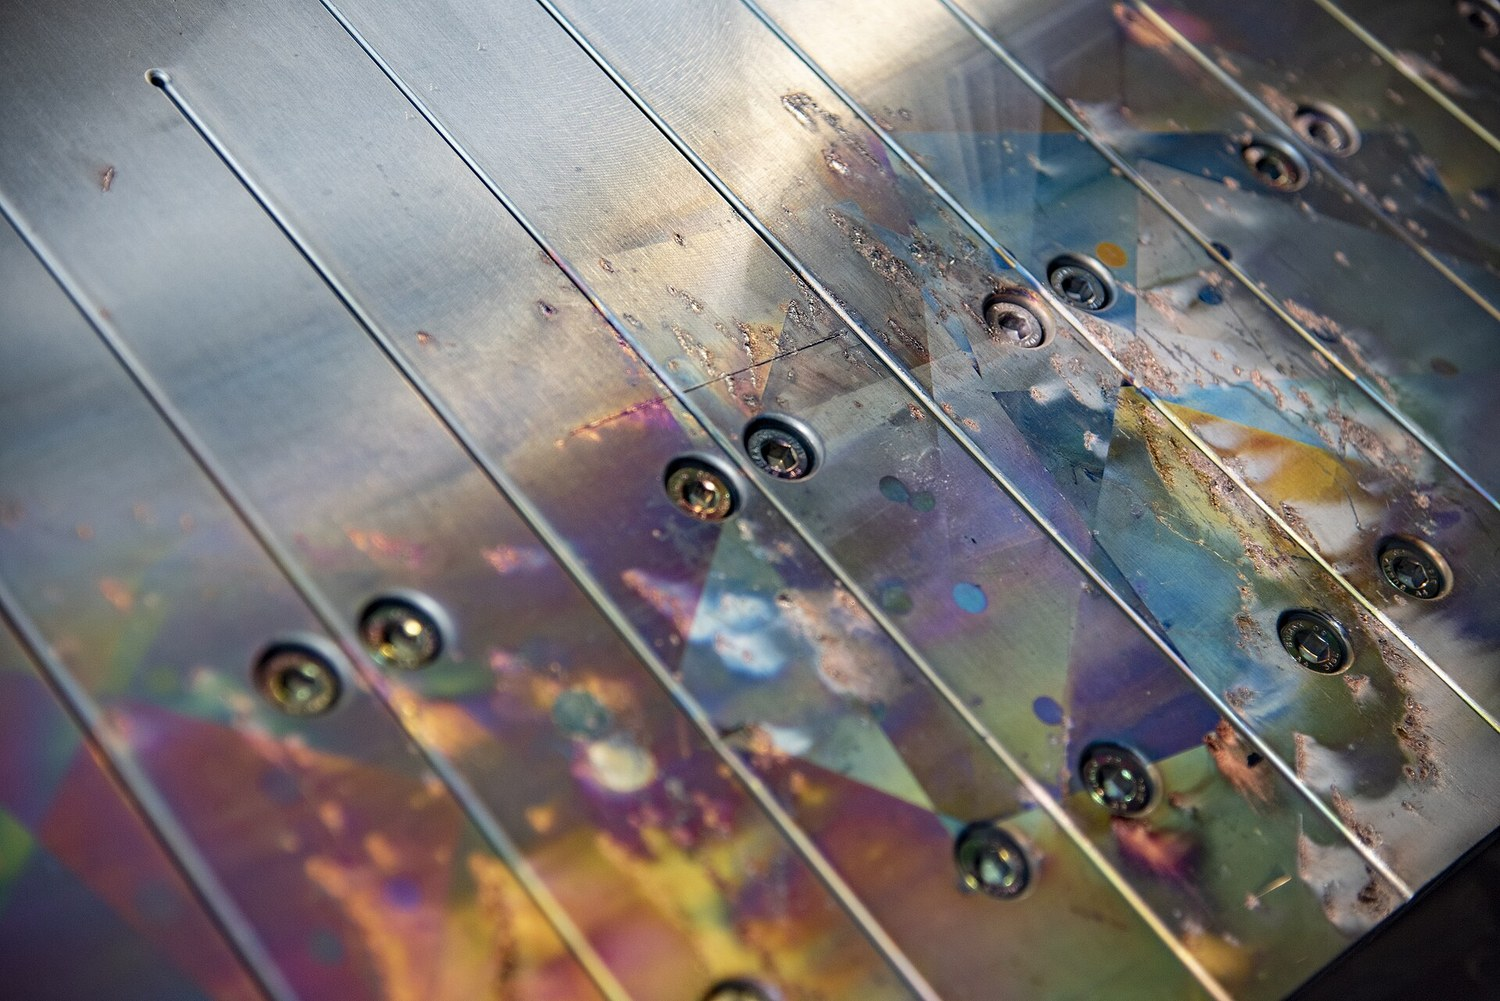
\includegraphics[width=0.72\textwidth]{../figures/v_pfc_erosion.jpg}
\caption{破裂的代价留在壁上：这块面向等离子体部件表面被侵蚀、又在别处再沉积了一层。本节把力、热与电子三笔账分别算完，最后都落在这张照片所示的那种表面损伤上。}
\label{fig:photo-appv2}
\figsource{Christophe Roux / CEA IRFM，CC BY 4.0（Wikimedia Commons）}
\end{figure}

\section{破裂的后果：力、热与电子三本账}
\label{sec:app-v-consequence}

破裂把三样东西交给壁：热储能、电流，以及由电流衍生出来的电磁力与高能电子。这三本账的量级
完全不同，所以要分开算。

\textbf{热账。} 热猝灭把热储能 $W_{\mathrm{th}}=371.4\ \mathrm{MJ}$（附录 U 的 D1 点）在
约 $1\ \mathrm{ms}$ 内交出去，瞬时功率 $371.4\ \mathrm{GW}$。若均匀摊在
$800\ \mathrm{m^2}$ 的第一壁上，功率密度是 $464.25\ \mathrm{MW/m^2}$，$1\ \mathrm{ms}$
内的能量密度是 $0.4642\ \mathrm{MJ/m^2}$。与附录 N.5 的瞬态热负荷口径（ELM 把
$1\ \mathrm{MJ/m^2}$ 在 $0.3\ \mathrm{ms}$ 内砸到靶板上）相比，这个数是「同一量级但更慢」。
把能量密度压到 $1\ \mathrm{MJ/m^2}$ 以下需要的受热面积是

\begin{equation}
A \ge \frac{W_{\mathrm{th}}}{1\ \mathrm{MJ/m^2}} = 371.4\ \mathrm{m^2}
\label{eq:app-v-qwall}
\end{equation}

也就是说：$371.4\ \mathrm{MJ}$ 必须被「摊开」，否则局部就会超过材料的瞬态损伤阈值。这正是
破裂缓解系统（V.6）存在的第一个理由。

\textbf{力账。} 电流猝灭期间，开磁力线把一部分电流引到壁上，形成晕电流。取常见的量级
$I_{\mathrm{halo}}=0.3I_{\mathrm p}=4.5\ \mathrm{MA}$，环向峰化因子取 2，则不对称部分约
$1.5\ \mathrm{MA}$。用一个玩具几何估算它受到的力（见本节的简化声明）：

\begin{equation}
F \approx I_{\mathrm{asym}}\,B_t\,L
= 1.5\times10^{6}\times5.3\times10
= 79.5\ \mathrm{MN}
\label{eq:app-v-force}
\end{equation}

其中取电流路径 $L=10\ \mathrm{m}$、环向场 $B_t=5.3\ \mathrm{T}$。$79.5\ \mathrm{MN}$ 的
量级与真空室和支撑结构的设计载荷相当，所以晕电流是结构设计的控制载荷之一。它不是「电流
乘时间」，而是「电流乘磁场乘几何」。

\textbf{电子账。} 电流猝灭把电子尾巴推成逃逸电子，束可以带着几 MA 电流继续跑，能量与热账
同量级，但落点要集中得多：$26.0\ \mathrm{MJ}$ 落在 $0.1\ \mathrm{m^2}$ 上是
$259.9\ \mathrm{MJ/m^2}$，比热账的 $0.4642\ \mathrm{MJ/m^2}$ 高两个多量级。下一节专门算
这本账。

\begin{table}[htbp]
\centering
\small
\caption{破裂的三本账。热账决定缓解系统要「摊开」多少面积，力账决定结构设计，电子账决定
为什么必须避免逃逸束形成。}
\label{tab:app-v-accounts}
\begin{tabular}{@{}p{1.9cm}p{3.4cm}p{3.4cm}p{3.4cm}@{}}
\toprule
账 & 数字 & 对照 & 结论 \\
\midrule
热账 & $371.4\ \mathrm{MJ}$；$464.25\ \mathrm{MW/m^2}$（$1\ \mathrm{ms}$、$800\ \mathrm{m^2}$） & 钨的瞬态阈值 $\sim1\ \mathrm{MJ/m^2}$（附录 N.5） & 必须摊到 $371.4\ \mathrm{m^2}$ 以上，否则局部熔融 \\
力账 & $I_{\mathrm{halo}}=4.5\ \mathrm{MA}$；力约 $79.5\ \mathrm{MN}$ & 真空室与支撑按几十至一百 MN 量级设计 & 晕电流是结构设计的控制载荷 \\
电子账 & $26.0\ \mathrm{MJ}$；$0.1\ \mathrm{m^2}$ 上 $259.9\ \mathrm{MJ/m^2}$ & 与热账同量级，但落点集中两个量级 & 逃逸束是唯一「点状」的失效模式 \\
\bottomrule
\end{tabular}

\end{table}

\textbf{本节声明：} 力账用的是玩具几何 $F\approx I_{\mathrm{asym}}B_tL$，它假定不对称
晕电流沿一条长约 $10\ \mathrm{m}$ 的路径在均匀环向场中流动；真实载荷要用三维真空室涡流
模型，本附录只取量级。

{\footnotesize
\textbf{出处：} 晕电流与电磁载荷、热猝灭的量级参照 Hender 等（2007）\textit{Nucl.\
Fusion} \textbf{47}, S128 与 Wesson《Tokamaks》第 4 版第 14 章。
瞬态热负荷的材料口径与
附录 N.5 一致（Loarte 等 2007 综述）。三本账的数值为本书自拟并独立复算。
}

\section{逃逸电子：Dreicer 场、雪崩与 26 MJ}
\label{sec:app-v-runaway}

电子在环向电场里被加速，同时被碰撞拖曳。两种作用的分界由两个场给出。第一个是
\textbf{Dreicer 场}：电场强到能与电子的碰撞摩擦相比时，整个电子分布开始被拉走。

\begin{equation}
E_D = \frac{n e^3 \ln\Lambda}{4\pi\varepsilon_0^2 k_B T}
= 44.3\ \mathrm{V/m}
\qquad
(n=10^{20}\ \mathrm{m^{-3}},\ T=1\ \mathrm{keV},\ \ln\Lambda=17)
\label{eq:app-v-ed}
\end{equation}

第二个是\textbf{临界场}：只需高能尾巴逃逸的场，它比 $E_D$ 小一个因子 $k_BT/m_ec^2$。

\begin{equation}
E_c = E_D\,\frac{k_B T}{m_e c^2} = 0.08668\ \mathrm{V/m},
\qquad
\frac{E_D}{E_c} = \frac{m_e c^2}{k_B T} = 511
\label{eq:app-v-ec}
\end{equation}

现在算电流猝灭期的环向场。$T_e=10\ \mathrm{eV}$ 的猝灭等离子体对应
$V_{\mathrm{loop}}=2600\ \mathrm{V}$（表 \ref{tab:app-v-cq}），于是

\begin{equation}
E_{\mathrm{tor}} = \frac{V_{\mathrm{loop}}}{2\pi R}
= \frac{2600}{2\pi\times6.2} = 66.74\ \mathrm{V/m}
\label{eq:app-v-eloop}
\end{equation}

三个场排在一起就是逃逸电子的全部故事：$E_c=0.08668\ \mathrm{V/m}$，
$E_{\mathrm{tor}}=66.74\ \mathrm{V/m}$，$E_D=4430\ \mathrm{V/m}$（$10\ \mathrm{eV}$ 口径）。
因为 $E_{\mathrm{tor}}/E_c=769.9$，尾巴会大量逃逸；又因为
$E_{\mathrm{tor}}/E_D=0.01507$，主体电子仍被碰撞拖住，不会整体被拉走。

\begin{table}[htbp]
\centering
\small
\caption{逃逸电子的三个特征场（$n=10^{20}\ \mathrm{m^{-3}}$、$\ln\Lambda=17$；$E_D$ 按
$T_e=10\ \mathrm{eV}$ 折算）。$E_c<E_{\mathrm{tor}}\ll E_D$ 正是「尾巴逃逸、主体不动」的
区间。}
\label{tab:app-v-fields}
\begin{tabular}{@{}p{3.4cm}p{2.2cm}p{2.8cm}p{3.6cm}@{}}
\toprule
场 & 数值 [V/m] & 与 $E_{\mathrm{tor}}$ 之比 & 含义 \\
\midrule
$E_c$（临界场） & 0.08668 & $E_{\mathrm{tor}}/E_c=769.9$ & 超过它就出现逃逸电子 \\
$E_{\mathrm{tor}}$（猝灭期环向场） & 66.74 & 1 & 由 $V_{\mathrm{loop}}=2600\ \mathrm{V}$ 与 $2\pi R$ 决定 \\
$E_D$（Dreicer 场，$10\ \mathrm{eV}$） & 4430 & $E_{\mathrm{tor}}/E_D=0.01507$ & 不到它的 2\%：主体电子仍被拖住 \\
\bottomrule
\end{tabular}

\end{table}

逃逸电子一旦出现，就会\textbf{雪崩}：逃逸电子与背景电子碰撞时，把后者也踢进逃逸区，数目
按指数增长。忽略拖曳与同步辐射的上界由 $e$ 折时间给出：

\begin{equation}
\tau_{\mathrm{av}} = \frac{m_e c\,\ln\Lambda}{e E_{\mathrm{tor}}}
= 0.4342\ \mathrm{ms}
\label{eq:app-v-avalanche}
\end{equation}

$40\ \mathrm{ms}$ 就是这个时间尺度的 $92.12$ 倍，放大倍数 $e^{92.12}\approx1.021\times10^{40}$。
结论很硬：种子电子有多少并不重要，限制雪崩的只有「电流通道能提供多少电流」。于是要算束的
能量，只需问它能带多少电流：

\begin{equation}
N_{\mathrm{RE}} = \frac{I_{\mathrm{RE}}\,2\pi R}{e c} = 8.1104\times10^{18},
\qquad
W_{\mathrm{RE}} = N_{\mathrm{RE}}(\gamma-1)m_e c^2 = 25.9885\ \mathrm{MJ}
\label{eq:app-v-wre}
\end{equation}

取 $I_{\mathrm{RE}}=10\ \mathrm{MA}$、电子能量 $20\ \mathrm{MeV}$：$25.9885\ \mathrm{MJ}$
落在 $0.1\ \mathrm{m^2}$ 上是 $259.9\ \mathrm{MJ/m^2}$，落在 $10\ \mathrm{m^2}$ 上是
$2.599\ \mathrm{MJ/m^2}$。束的「散开程度」决定壁的死活。

靠提高密度能不能压住雪崩？$E_c$ 与 $n$ 成正比，要让
$E_c$ 追平 $E_{\mathrm{tor}}$ 需要

\begin{equation}
n_{\mathrm{supp}} = 7.699\times10^{22}\ \mathrm{m^{-3}} = 645\,n_G
\label{eq:app-v-nsupp}
\end{equation}

即 $645$ 倍的 Greenwald 密度，工程上不可能。把密度抬到 $10^{21}\ \mathrm{m^{-3}}$（已是
$8.378$ 倍 $n_G$）也才把 $E_c$ 抬到 $0.8668\ \mathrm{V/m}$，$E_{\mathrm{tor}}/E_c$ 仍有
$76.99$。更麻烦的是「快」帮不上忙，反而有害：

\begin{table}[htbp]
\centering
\small
\caption{电流猝灭时间与环向场（$L_p=1.33294\times10^{-5}\ \mathrm{H}$、
$I_{\mathrm p}=15\ \mathrm{MA}$、$2\pi R=2\pi\times6.2$）。要让
$E_{\mathrm{tor}}<E_c$ 需要 $\tau_{\mathrm{CQ}}=5.921\ \mathrm{s}$，比工程能接受的
$50$--$150\ \mathrm{ms}$ 长两个量级。}
\label{tab:app-v-cq}
\begin{tabular}{@{}p{2.6cm}p{2.6cm}p{3.0cm}p{3.4cm}@{}}
\toprule
$\tau_{\mathrm{CQ}}$ [s] & $E_{\mathrm{tor}}$ [V/m] & $E_{\mathrm{tor}}/E_c$（$n_e=10^{21}$） & 判断 \\
\midrule
0.01 & 513.3 & 592.1 & 快猝灭：雪崩最猛 \\
0.05 & 102.7 & 118.4 & 雪崩仍然很强 \\
0.10 & 51.33 & 59.21 & 工程上典型的猝灭时间 \\
0.20 & 25.66 & 29.60 & 仍远在 $E_c$ 之上 \\
0.50 & 10.27 & 11.84 & 接近但不够 \\
1.00 & 5.133 & 5.921 & 还要慢六倍 \\
\bottomrule
\end{tabular}

\end{table}

\begin{tip}{把电流拉得越快，雪崩越猛}{tip-app-v-runaway}
表 \ref{tab:app-v-cq} 的第一行与最后一行差两个量级：$\tau_{\mathrm{CQ}}$ 从
$1\ \mathrm{s}$ 缩到 $0.01\ \mathrm{s}$，环向场从 $5.133$ 升到 $513.3\ \mathrm{V/m}$。
所以「快」不是免费的。缓解系统的第一任务是把热储能辐射掉（表
\ref{tab:app-v-accounts} 的热账），第二任务是在逃逸电子形成之前把电流「安全地」交出去。
\end{tip}

{\footnotesize
\textbf{出处：} Dreicer 场的定义参照 Dreicer（1959）\textit{Phys.\ Rev.}
\textbf{115}, 238。
相对论临界场与逃逸条件参照 Connor \& Hastie（1975）\textit{Nucl.\
Fusion} \textbf{15}, 415。
雪崩的增长率与饱和参照 Rosenbluth \& Putvinski（1997）
\textit{Nucl.\ Fusion} \textbf{37}, 1355。本节的三个场、雪崩 $e$ 折时间与束能量估计为
本书自拟，量级 1 的精确系数归原文。
}

\begin{figure}[htbp]
\centering
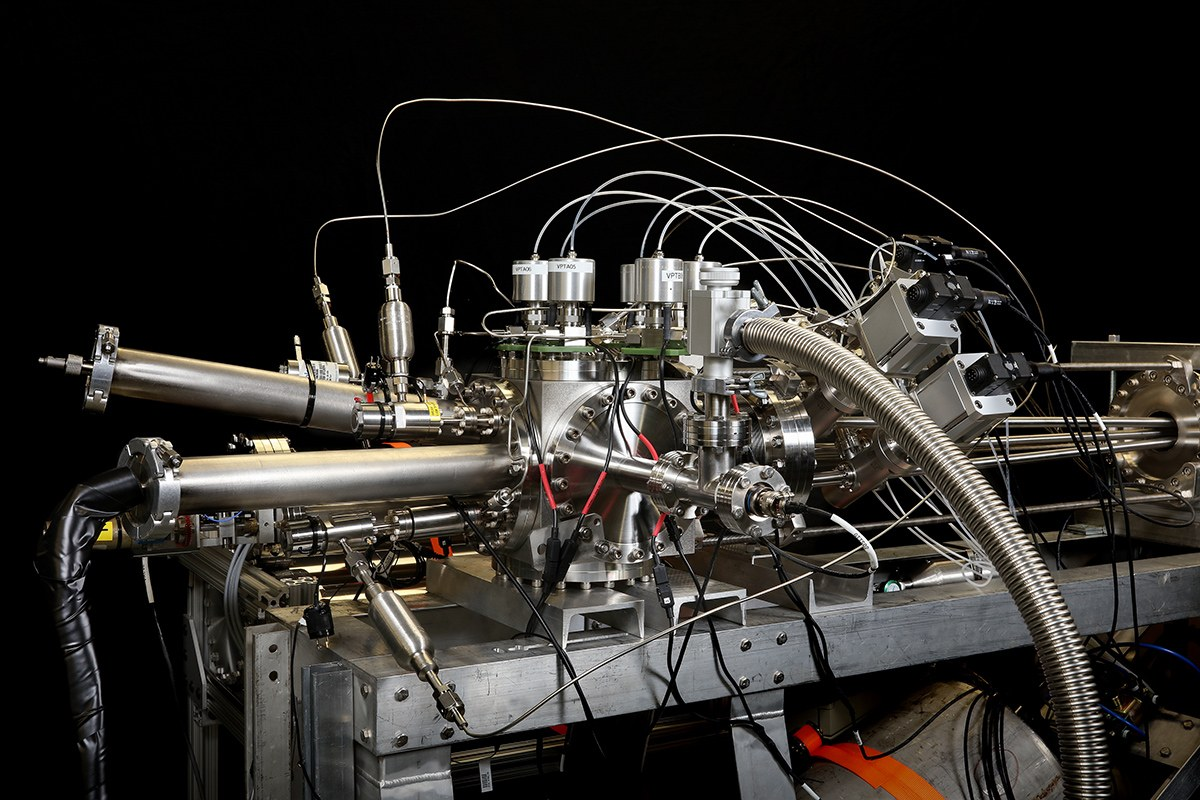
\includegraphics[width=0.78\textwidth]{../figures/v_spi_test_stand.jpg}
\caption{橡树岭国家实验室的碎裂弹丸试验台：把弹丸冻成柱、加速、在进入等离子体前碎成云，用来在几毫秒内把等离子体「淬灭」。这是缓解破裂、把电磁力与热流摊开的工程手段。}
\label{fig:photo-appv3}
\figsource{Oak Ridge National Laboratory，CC BY 2.0（Wikimedia Commons）}
\end{figure}

\section{避免、预测与缓解：把破裂当工程问题}
\label{sec:app-v-mitigation}

工程上把破裂拆成三个不同的动词：避免（avoidance）、预测（prediction）、缓解
（mitigation）。三者的目标不同，指标也不同。

\textbf{避免}是把工作点放在离极限足够远处。本书工作点的三个裕度是：
$n/n_G=83.78\%$（离密度极限 $16.22\%$）、$\beta_N=1.8627$（离无壁极限 $2.8$ 有
$33.475\%$ 的裕度）、误差场要校正到 $0.795\ \mathrm{mT}$ 以下（V.2）。这些都是「静态」的
裕度，靠运行前规划得到。

\textbf{预测}靠先兆。锁模是最可靠的先兆信号，而预警窗口必须覆盖「探测 $+$ 决策 $+$ 注入
$+$ 同化」这四步。对 JET 破裂原因的系统调查给出的窗口量级是 $10$--$100\ \mathrm{ms}$；
这是统计结果，不是本附录算出来的数——本附录能算的是「窗口里必须做完哪些事」（见表
\ref{tab:app-v-timeline} 的前两阶段）。

\textbf{缓解}要把两件事同时做完。第一件是把热储能辐射掉，需要的杂质原子数是

\begin{equation}
N_{\mathrm{imp}} = \frac{P_{\mathrm{rad}}}{n_e L_z} = 1.238\times10^{21}
\label{eq:app-v-impurity}
\end{equation}

取 $P_{\mathrm{rad}}=3.714\times10^{10}\ \mathrm{W}$（$371.4\ \mathrm{MJ}$ 在
$10\ \mathrm{ms}$ 内辐射掉）、$n_e=10^{21}\ \mathrm{m^{-3}}$、冷却率系数
$L_z=3\times10^{-32}\ \mathrm{W\,m^3}$（与附录 N 同口径）：$1.238\times10^{21}$ 个原子
占等离子体离子库存 $8.322\times10^{22}$ 的 $1.488\%$，折成 $300\ \mathrm{K}$ 气体是
$5.128\ \mathrm{Pa\,m^3}$。第二件是把电子密度抬到 $10^{21}\ \mathrm{m^{-3}}$ 以压低
$E_{\mathrm{tor}}/E_c$（V.5），需要 $8.322\times10^{23}$ 个粒子，即
$3.447\ \mathrm{kPa\,m^3}$ 的 $300\ \mathrm{K}$ 气体。

\begin{table}[htbp]
\centering
\small
\caption{破裂缓解的两项任务。第二项比第一项大 $672$ 倍，所以工程注入系统的规模是由「抬密度
压逃逸电子」决定的，而不是由「辐射热储能」决定的。}
\label{tab:app-v-mitigation}
\begin{tabular}{@{}p{2.4cm}p{2.8cm}p{2.6cm}p{3.4cm}@{}}
\toprule
任务 & 需要的粒子数 & 折成 $300\ \mathrm{K}$ 气体 & 说明 \\
\midrule
辐射掉热储能 & $1.238\times10^{21}$ & $5.128\ \mathrm{Pa\,m^3}$ & 占离子库存 $1.488\%$（$L_z=3\times10^{-32}$） \\
把密度抬到 $10^{21}$ & $8.322\times10^{23}$ & $3.447\ \mathrm{kPa\,m^3}$ & 压低 $E_{\mathrm{tor}}/E_c$，是注入量的驱动项 \\
\bottomrule
\end{tabular}

\end{table}

两项任务的账相差 $672$ 倍，这就解释了缓解系统的设计取向。现代装置用大量气体注入（MGI）
或破碎弹丸注入（SPI）把高 $Z$ 杂质（氖、氩）在几毫秒内送进等离子体，辐射掉能量，同时增加对逃逸
电子的拖曳。如果逃逸束已经形成，就只能靠环向场斜坡下降与有意激发的 MHD 活动把它散开。

破裂不是「事故」，而是运行空间的边界本身。一个装置能走多远，由「离破裂有多远」决定。

\begin{tip}{把简化声明写在明处}{tip-app-v-honest}
本附录有四处刻意的简化：(1) 晕电流力用玩具几何 $F\approx I_{\mathrm{asym}}B_tL$，真实
载荷要用三维真空室涡流模型。
(2) 猝灭期的电阻用 Spitzer 公式与 $Z_{\mathrm{eff}}=2$、
$\ln\Lambda=17$，而低温下电阻率会偏离 Spitzer。
(3) 雪崩只用 $e$ 折时间尺度
$\tau_{\mathrm{av}}$，量级 1 的系数见 Rosenbluth \& Putvinski（1997）。
(4) 杂质冷却率
取 $L_z=3\times10^{-32}\ \mathrm{W\,m^3}$，与附录 N 同口径，但 $L_z$ 随温度变化可达一个
量级。这些简化不影响结论的量级，但精确到 $10\%$ 的工程数必须用专门的代码。
\end{tip}

{\footnotesize
\textbf{出处：} 破裂预测的预警窗口与先兆统计参照 de Vries 等（2011）\textit{Nucl.\
Fusion} \textbf{51}, 053018（JET 破裂原因调查）。
缓解系统（MGI 与 SPI）的现状参照
Hollmann 等（2015）\textit{Phys.\ Plasmas} \textbf{22}, 021802 与 Hender 等（2007）。
两项任务的粒子数与气量账为本书自拟。
}

\section{六道估算练习}
\label{sec:app-v-problems}

\textbf{练习 1（$\beta$ 与 $\beta_N$）}
D1 点取 $n=10^{20}\ \mathrm{m^{-3}}$、$T=9.194\ \mathrm{keV}$、$B=5.3\ \mathrm{T}$、
$a=2.0\ \mathrm{m}$、$I_{\mathrm p}=15\ \mathrm{MA}$，求 $\beta$ 与 $\beta_N$，并回答离
无壁极限还有多少裕度。

\textbf{解答}：由式 \eqref{eq:app-v-betan}，$p=2nk_BT=2.946\times10^{5}\ \mathrm{Pa}$、
$B^2/2\mu_0=1.118\times10^{7}\ \mathrm{Pa}$，得 $\beta=2.6359\%$；
$\beta_N=2.6359\times2.0\times5.3/15=1.8627$。离无壁极限 $2.8$ 的裕度是
$(2.8-1.8627)/2.8=33.475\%$。注意这是\textbf{相对极限}的裕度，不是「还能把温度提高
33.475\%」（温度与 $\beta$ 成正比，但提高温度会改变功率平衡）。

\textbf{练习 2（晕电流的力）}
取 $I_{\mathrm{halo}}=0.3I_{\mathrm p}$、环向峰化因子 $2$、$B_t=5.3\ \mathrm{T}$、电流
路径 $L=10\ \mathrm{m}$，估算不对称晕电流受到的力。

\textbf{解答}：$I_{\mathrm{halo}}=4.5\ \mathrm{MA}$，不对称部分约
$I_{\mathrm{halo}}/3=1.5\ \mathrm{MA}$；由式 \eqref{eq:app-v-force}，
$F\approx1.5\times10^{6}\times5.3\times10=79.5\ \mathrm{MN}$。量级与真空室设计载荷相当，
所以晕电流必须进结构载荷清单。

\textbf{练习 3（电流猝灭时间）}
取 $L_p=\mu_0R[\ln(8R/a)-2+l_i/2]$（$l_i=1$）、$T_e=10\ \mathrm{eV}$、
$Z_{\mathrm{eff}}=2$、$\ln\Lambda=17$，求等离子体电阻、猝灭时间与环电压。

\textbf{解答}：$L_p=1.33294\times10^{-5}\ \mathrm{H}$；
$\eta=5.2\times10^{-5}\times2\times17/10^{1.5}=5.591\times10^{-5}\ \Omega\,\mathrm{m}$；
$R_p=\eta\,2\pi R/(\pi a^2)=1.733\times10^{-4}\ \Omega$；
$\tau_{\mathrm{CQ}}=L_p/R_p=76.9074\ \mathrm{ms}$；
$V_{\mathrm{loop}}=I_{\mathrm p}R_p=2600\ \mathrm{V}$。这个时间落在表
\ref{tab:app-v-timeline} 给的 $50$--$150\ \mathrm{ms}$ 区间内。

\textbf{练习 4（三个电场）}
$n=10^{20}\ \mathrm{m^{-3}}$、$\ln\Lambda=17$，求 $T=1\ \mathrm{keV}$ 的 $E_D$ 与
$E_c$；再取猝灭期 $E_{\mathrm{tor}}=66.74\ \mathrm{V/m}$，判断它与两个场的关系。

\textbf{解答}：式 \eqref{eq:app-v-ed} 给 $E_D=44.3\ \mathrm{V/m}$，式
\eqref{eq:app-v-ec} 给 $E_c=0.08668\ \mathrm{V/m}$（比值 $511$，正好是
$m_ec^2/k_BT$）。$E_{\mathrm{tor}}/E_c=769.9$，所以逃逸电子必然出现；
$E_{\mathrm{tor}}/E_D=0.01507$（$E_D$ 按 $10\ \mathrm{eV}$ 折算是 $4430\ \mathrm{V/m}$），
所以主体电子不会被整体拉走。这就是「尾巴逃逸、主体不动」的定量含义。

\textbf{练习 5（逃逸束的能量）}
$10\ \mathrm{MA}$ 的逃逸束、电子平均能量 $20\ \mathrm{MeV}$，求束内电子数与总能量；若束
落在 $0.1\ \mathrm{m^2}$ 上，能量密度是多少？

\textbf{解答}：由式 \eqref{eq:app-v-wre}，
$N_{\mathrm{RE}}=10\times10^{6}\times2\pi\times6.2/(e c)=8.1104\times10^{18}$；
$W_{\mathrm{RE}}=N_{\mathrm{RE}}\times20\ \mathrm{MeV}=25.9885\ \mathrm{MJ}$。
落在 $0.1\ \mathrm{m^2}$ 上是 $259.9\ \mathrm{MJ/m^2}$，比热账的
$0.4642\ \mathrm{MJ/m^2}$ 高两个多量级。这就是「逃逸束是点状失效模式」的算术含义。

\textbf{练习 6（壁时间与反馈带宽）}
取 $\delta=3\ \mathrm{cm}$、$d=1\ \mathrm{m}$，求不锈钢（$\sigma=1.4\times10^6$）与铜
（$\sigma=5.8\times10^7$）的壁时间，并给出反馈带宽要求。

\textbf{解答}：由式 \eqref{eq:app-v-tauw}，不锈钢给 $\tau_w=52.7788\ \mathrm{ms}$、铜给
$2.18655\ \mathrm{s}$（相差 $41.428$ 倍）。RWM 增长率由式 \eqref{eq:app-v-rwm} 得
$18.947\ \mathrm{s^{-1}}$，反馈带宽要按 $\tau_w/10$ 设计，即 $189.47\ \mathrm{s^{-1}}$。

\section{来源、分级与版权说明}
\label{sec:app-v-source}

\begingroup\small
本附录使用的公式类型、结论与题型均有明确出处；所有数值、表格与文字自拟，并由
\texttt{tools/\allowbreak{}calc/\allowbreak{}appV\_calc.py} 独立复算。参考文献只给书名、作者、年份与卷期页。

\begin{table}[htbp]
\centering
\small
\caption{本附录的借鉴来源与自拟部分对照表。所有量级 1 的精确系数、实验定标与工程设计值均
归原始文献，本附录只借用物理结论与公式形式。}
\label{tab:app-v-source}
\begin{tabular}{@{}p{1.4cm}p{5.4cm}p{4.0cm}p{3.4cm}@{}}
\toprule
小节 & 借鉴来源 & 借鉴内容 & 本书自拟部分 \\
\midrule
V.1 & Wesson《Tokamaks》4th ed. 第 14 章；Freidberg《Plasma Physics and Fusion Energy》第 13 章；Hender 等（2007） & 三条运行极限的分类、破裂时间线 & 工作点上的 $\beta$、$\beta_N$、$n_G$ 与全部表格数值 \\
V.2 & Hender 等（2007）；Fitzpatrick（1993） & 误差场穿透、锁模与校正线圈 & 真空折算算例（式 \eqref{eq:app-v-vacuum}）与阈值折算 \\
V.3 & Troyon 等（1984）；Chu \& Okabayashi（2010）；Freidberg《Ideal MHD》 & $\beta_N$ 定义与极限区间、RWM 与反馈 & $\tau_w$ 算例、增长率与反馈带宽要求 \\
V.4 & Hender 等（2007）；Wesson 第 14 章 & 晕电流与电磁载荷、热猝灭量级 & 三本账的计算（玩具几何已声明） \\
V.5 & Dreicer（1959）；Connor \& Hastie（1975）；Rosenbluth \& Putvinski（1997） & Dreicer 场、临界场、雪崩 & 三个场的数值算例、$e$ 折时间与束能量 \\
V.6 & de Vries 等（2011）；Hollmann 等（2015）；Hender 等（2007） & 先兆统计与缓解系统现状 & 两项任务的粒子数与气量账 \\
V.7 & 本书自拟 & 六道估算题的题型 & 全部数字来自 \texttt{tools/\allowbreak{}calc/\allowbreak{}appV\_calc.py} \\
\bottomrule
\end{tabular}

\end{table}

\textbf{三条「不复制」约定：}
(1) 不复制任何教材或论文的表格数值——本附录每一张表的数字都能用
\texttt{tools/\allowbreak{}calc/\allowbreak{}appV\_calc.py} 从同一组输入复算。
(2) 不复制原文文字——所有叙述重新组织，并把简化与适用条件写在正文与语义盒里。
(3) 不把实验定标写成「公式」——凡属统计或工程经验的数字（预警窗口、材料阈值、注入系统
规模）都显式标注为经验值。

\textbf{与相邻附录的关系：} 附录 M 给出运行极限的「面」，附录 N 给出边界与瞬态热负荷，
附录 S 给出约束定标，附录 T 给出磁岛几何，附录 U 给出增益与点火。本附录把「运行空间什么
时候被撞破」补上：五条路径（表 \ref{tab:app-v-limits}）、一条时间线（表
\ref{tab:app-v-timeline}）、三本账（表 \ref{tab:app-v-accounts}）。六者用的是同一组工作点，
可以互相代入验算。
\endgroup
